% Recruiting flyer for IMSE 774, Fall 2026.
% Build with: pdflatex flyer.tex  (needs flyer/banner.pdf from banner.py)
\documentclass[10pt]{article}

\usepackage[letterpaper,left=0.55in,right=0.55in,top=1.95in,bottom=1.05in]{geometry}
\usepackage[T1]{fontenc}
\usepackage[utf8]{inputenc}
\usepackage[sfdefault]{roboto}
\usepackage{microtype}
\usepackage{xcolor}
\usepackage{tikz}
\usepackage{tcolorbox}
\usepackage{fontawesome5}
\usepackage{qrcode}
\usepackage{graphicx}
\usepackage{enumitem}
\usepackage{paracol}
\tcbuselibrary{skins}
\usetikzlibrary{calc}

\definecolor{ndsugreen}{HTML}{005643}
\definecolor{ndsudark}{HTML}{00382C}
\definecolor{ndsugold}{HTML}{FFC72C}
\definecolor{ink}{HTML}{1F2421}
\definecolor{slate}{HTML}{5A6560}
\definecolor{mist}{HTML}{EEF3F1}

\pagestyle{empty}
\setlength{\parindent}{0pt}
\color{ink}

% ---------------------------------------------------------------- helpers ----
\newcommand{\heading}[1]{%
  \vspace{2pt}%
  {\color{ndsugreen}\bfseries\fontsize{11}{13}\selectfont #1}%
  \par\vspace{1pt}%
  {\color{ndsugold}\rule{\linewidth}{1.2pt}}%
  \par\vspace{4pt}%
}

% One "what you'll learn" block: gold lead-in, then the detail.
\newcommand{\topicblock}[2]{%
  {\bfseries\color{ndsugreen}#1}\par
  \vspace{0.5pt}{\color{slate}\fontsize{8.6}{10.4}\selectfont #2}\par
  \vspace{4.5pt}%
}

% A labelled fact row inside the sidebar.
\newcommand{\fact}[2]{%
  {\fontsize{7.6}{9}\selectfont\bfseries\color{ndsugreen}\MakeUppercase{#1}}\par
  {\fontsize{9}{10.8}\selectfont\raggedright #2\par}\vspace{4.5pt}%
}

\begin{document}

% -------------------------------------------------------- page furniture ----
% Both bands are drawn from a single overlay at the top of the document. They
% are anchored to the page rather than the text flow, so putting the footer here
% keeps it on page one instead of letting it break to a second page once the
% body fills the text block.
\begin{tikzpicture}[remember picture,overlay]
  \fill[ndsugreen]
    (current page.north west) rectangle
    ($(current page.north east)+(0,-1.62in)$);
  \fill[ndsugold]
    ($(current page.north west)+(0,-1.62in)$) rectangle
    ($(current page.north east)+(0,-1.68in)$);

  % Course identity, left aligned to the text block.
  \node[anchor=north west,inner sep=0pt] at ($(current page.north west)+(0.55in,-0.34in)$) {%
    \begin{minipage}{4.9in}
      \color{ndsugold}\fontsize{10.5}{12}\selectfont\bfseries
      IMSE 774\par
      \vspace{3pt}
      \color{white}\fontsize{34}{37}\selectfont\bfseries
      Neural Networks\par
      \vspace{5pt}
      \color{white}\fontsize{11.5}{14}\selectfont\mdseries
      Fall 2026 \enspace\textbullet\enspace 3 credits \enspace\textbullet\enspace
      North Dakota State University
    \end{minipage}%
  };

  % Decorative network sketch, right side of the band.
  \begin{scope}[shift={($(current page.north east)+(-1.6in,-0.82in)$)}]
    \foreach \i in {0,1,2} { \coordinate (a\i) at (0, {0.42-0.42*\i}); }
    \foreach \i in {0,1,2,3} { \coordinate (b\i) at (0.62, {0.63-0.42*\i}); }
    \foreach \i in {0,1,2,3} { \coordinate (c\i) at (1.24, {0.63-0.42*\i}); }
    \foreach \i in {0,1} { \coordinate (d\i) at (1.86, {0.21-0.42*\i}); }
    \foreach \i in {0,1,2} \foreach \j in {0,1,2,3}
      \draw[ndsugold!45,line width=0.35pt] (a\i) -- (b\j);
    \foreach \i in {0,1,2,3} \foreach \j in {0,1,2,3}
      \draw[ndsugold!30,line width=0.35pt] (b\i) -- (c\j);
    \foreach \i in {0,1,2,3} \foreach \j in {0,1}
      \draw[ndsugold!45,line width=0.35pt] (c\i) -- (d\j);
    \foreach \i in {0,1,2} \fill[white] (a\i) circle (2.4pt);
    \foreach \i in {0,1,2,3} \fill[ndsugold] (b\i) circle (2.4pt);
    \foreach \i in {0,1,2,3} \fill[ndsugold] (c\i) circle (2.4pt);
    \foreach \i in {0,1} \fill[white] (d\i) circle (2.4pt);
  \end{scope}

  % ---------------------------------------------------------- footer band ----
  \fill[ndsugold]
    ($(current page.south west)+(0,0.80in)$) rectangle
    ($(current page.south east)+(0,0.86in)$);
  \fill[ndsugreen]
    (current page.south west) rectangle
    ($(current page.south east)+(0,0.80in)$);

  \node[anchor=north west,inner sep=0pt] at ($(current page.south west)+(0.55in,0.62in)$) {%
    \begin{minipage}{4.4in}
      \color{white}\fontsize{11}{13}\selectfont\bfseries Harun Pirim, PhD\par
      \vspace{2.5pt}
      \color{white}\fontsize{8.8}{11}\selectfont\mdseries
      Industrial and Manufacturing Systems Engineering\par
      \vspace{1.5pt}
      \color{ndsugold}\fontsize{8.8}{11}\selectfont
      \faEnvelope\enspace harun.pirim@ndsu.edu \quad
      \faPhone*\enspace (701) 231-7285 \quad
      \faMapMarker*\enspace Offerdahl 106
    \end{minipage}%
  };

  \node[anchor=north east,inner sep=0pt] at ($(current page.south east)+(-0.55in,0.60in)$) {%
    \begin{minipage}{2.3in}
      \raggedleft
      \color{ndsugold}\fontsize{9.5}{12}\selectfont\bfseries
      Questions? Email me.\par
      \vspace{2pt}
      \color{white}\fontsize{8.4}{10.5}\selectfont\mdseries
      Register through NDSU\\Campus Connection.
    \end{minipage}%
  };
\end{tikzpicture}

% ------------------------------------------------------------------- hook ----
{\fontsize{12.5}{15.5}\selectfont\bfseries\color{ndsugreen}\raggedright
Derive deep learning from first principles, implement every piece in PyTorch,
and finish the semester with a working model on a problem you chose.\par}

\vspace{9pt}

% --------------------------------------------------------------- two cols ----
\columnratio{0.615}
\begin{paracol}{2}

\heading{What You Will Learn}

\topicblock{Foundations}{Shallow and deep networks, what depth actually buys
you, backpropagation worked through by hand, and initialization that keeps
gradients alive.}

\topicblock{Training that works}{Loss functions from maximum likelihood,
stochastic gradient descent and Adam, regularization, and how to measure
generalization honestly.}

\topicblock{Modern architectures}{Convolutional networks, transformers and the
attention mechanism, large language models, and graph neural networks for
relational data.}

\topicblock{Generative models}{Variational autoencoders, generative adversarial
networks, and the diffusion models behind today's image generators.}

\vspace{1pt}
\heading{How the Course Runs}

{\fontsize{8.8}{10.9}\selectfont
\begin{itemize}[leftmargin=11pt,itemsep=2.4pt,topsep=0pt,parsep=0pt,partopsep=0pt]
  \item Every topic pairs the mathematics with a runnable PyTorch
        implementation --- no black boxes.
  \item Roughly weekly assignments, distributed and submitted as Jupyter
        notebooks.
  \item A semester project on a real problem. Bring your own research data and
        leave with a result you can publish.
  \item Read and present a recent paper, then argue about where the field goes
        next.
\end{itemize}\par}

\vspace{5pt}
\heading{Who Should Enroll}

{\fontsize{8.8}{10.9}\selectfont
Graduate students in \textbf{engineering} and \textbf{computer science}, and
anyone whose research runs on data. The only prerequisite is graduate standing
--- no previous machine learning course is required. You should be comfortable
with linear algebra, calculus, and basic Python; the course builds the rest.\par}

% ------------------------------------------------------------- side column ----
\switchcolumn

\begin{tcolorbox}[
  enhanced, sharp corners, boxrule=0pt, frame hidden,
  colback=mist, borderline west={2.6pt}{0pt}{ndsugold},
  left=9pt, right=8pt, top=9pt, bottom=7pt,
]
\fact{Meets}{Tuesday \& Thursday\\12:30--1:45 p.m.}
\fact{Term}{August 25 -- December 10, 2026}
\fact{Open to}{All graduate students}
\fact{Prerequisite}{Graduate standing}
\fact{Software}{Python and PyTorch.\\Google Colab is fine --- nothing to
install.}
{\fontsize{7.6}{9}\selectfont\bfseries\color{ndsugreen}TEXTBOOK}\par
{\fontsize{9}{10.8}\selectfont Prince, \textit{Understanding Deep Learning},
MIT Press, 2024 --- \textbf{free online}.}
\end{tcolorbox}

\vspace{8pt}

\begin{center}
  \qrcode[height=1.15in,level=M]{https://harunpirim.github.io/IMSE774-NeuralNetworks/}\par
  \vspace{5pt}
  {\fontsize{8.4}{10}\selectfont\bfseries\color{ndsugreen}
  Syllabus, schedule, and every\\lecture note --- free and open.\par}
  \vspace{2pt}
  {\fontsize{7.2}{8.6}\selectfont\color{slate}
  harunpirim.github.io/\\IMSE774-NeuralNetworks\par}
\end{center}

\end{paracol}

% ----------------------------------------------------------- banner figure ----
% Caption and plot travel together so \vfill cannot break between them.
\vfill
\begin{minipage}{\linewidth}
  {\color{ndsugreen}\fontsize{8.4}{10}\selectfont\bfseries\raggedright
  One hidden layer, one nonlinearity, and enough units: the universal
  approximation theorem, made concrete in week 3.\par}
  \vspace{3pt}
  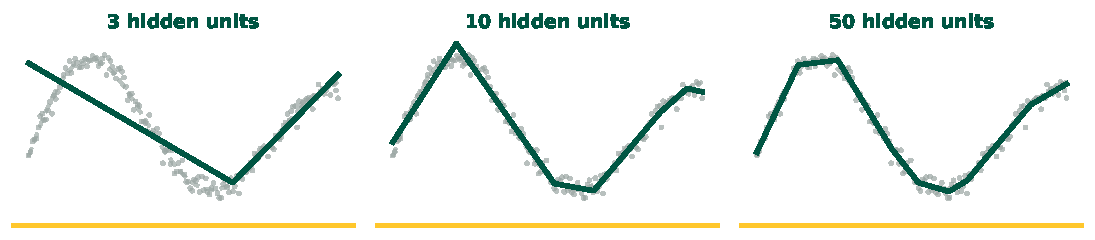
\includegraphics[width=\linewidth]{banner.pdf}
\end{minipage}

\end{document}
